\subsection{Implicit upwind scheme parallel algorithm} \label{s:general-approach:implicit-upwind-parallel-algorithm}
	Implicit upwind scheme dependencies are shown in Figure \ref{fig:stencil:implicit-upwind}. According to the \gls{stencil} in order to calculate new point at time $n+1$ this scheme requires previous or next (depending on sign of \gls{CFL}) point of a grid from time $n+1$ and current point at time $n$. It means that each of the processors requires one value from previous processor (in terms of their ids) to start calculations. Figure \ref{fig:communication:implicit-upwind} presents discussed earlier communication between processors. Transfered $f_{lmax}^{n+1}$ relates to the last point in the local grid calculated at time $n+1$, where $lmax$ is determined as shown in Listing \ref{lst:fragmentation}.
	\begin{figure}[!htbp]
		\centering
		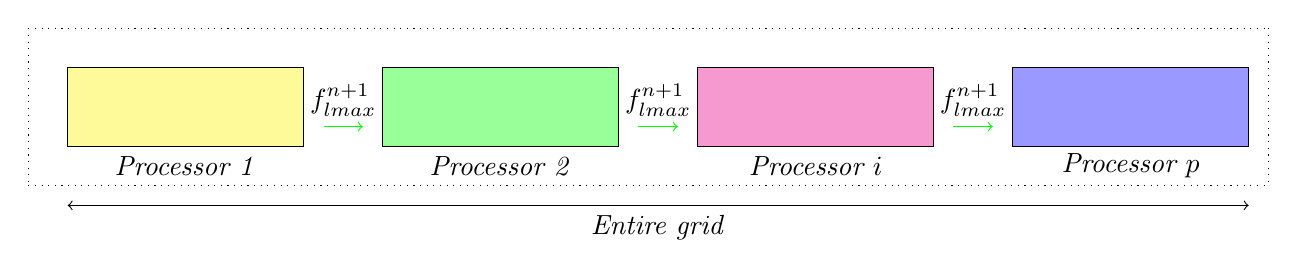
\begin{tikzpicture}[scale=1.0]
			\draw[dotted] (-0.5,-0.5) -- (15.25,-0.5);
			\draw[dotted] (-0.5, 1.5) -- (15.25, 1.5);
			\draw[dotted] (-0.5, 1.5) -- (-0.5, -0.5);
			\draw[dotted] (15.25, 1.5) -- (15.25, -0.5);
			\filldraw[fill=yellow!40!white, draw=black] (0,0) rectangle (3,1);
			\filldraw[fill=green!40!white, draw=black] (4,0) rectangle (7,1);
			\filldraw[fill=magenta!40!white, draw=black] (8,0) rectangle (11,1);
			\filldraw[fill=blue!40!white, draw=black] (12,0) rectangle (15,1);
			\node[align=right] at (1.5, -0.25) {\emph{Processor 1}};
			\node[align=right] at (5.5, -0.25) {\emph{Processor 2}};
			\node[align=right] at (9.5, -0.25) {\emph{Processor $i$}};
			\node[align=right] at (13.5, -0.25) {\emph{Processor $p$}};
			\draw [->][green] (3.25, 0.25) -- node [midway, above, sloped, black] {$f_{lmax}^{n+1}$} (3.75, 0.25);
			\draw [->][green] (7.25, 0.25) -- node [midway, above, sloped, black] {$f_{lmax}^{n+1}$} (7.75, 0.25);
			\draw [->][green] (11.25, 0.25) -- node [midway, above, sloped, black] {$f_{lmax}^{n+1}$} (11.75, 0.25);
			\draw[<->] (0,-0.75) -- node [midway, below, sloped, black] {\emph{Entire grid}} (15,-0.75);
		\end{tikzpicture}
		\caption{Communication between processors in parallel implicit upwind schema for $\gls{CFL} > 0$.}
		\label{fig:communication:implicit-upwind}
	\end{figure}
	Parallel calculations for implicit upwind schema are visualized in Figure \ref{fig:visualization:implicit-upwind}. This scheme depends on values from new solution so boundaries are sent between neighboring processors after full iteration through local grids in previous processor. We can assume that all the processors will be working simultaneously after full iteration of through grid. Some of those will be calculating local grids at time $n$ and others at $n+1$ depending on their ids.
	\begin{figure}[!htbp]
		\centering
		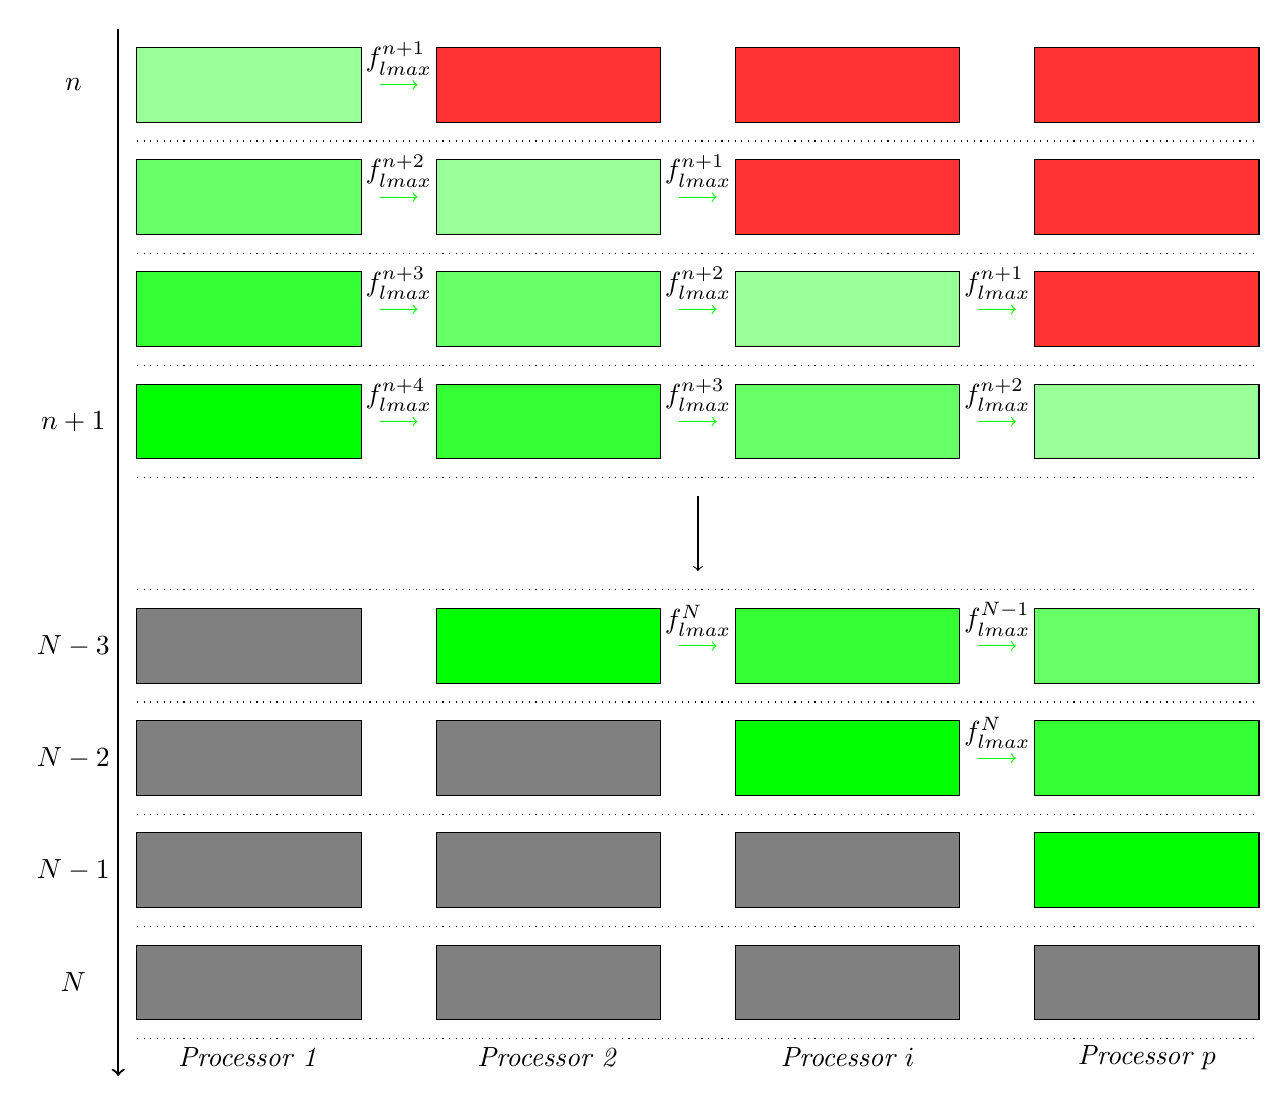
\begin{tikzpicture}[scale=0.95]
			\draw [->] [black, thick] (-.25, 0.25) -- (-.25, -13.75);
			\node[black] at (-0.85, -0.5) {$n$};
			\draw [->][green] (3.25, -0.5) -- node [midway, above, sloped, black] {$f_{lmax}^{n+1}$} (3.75, -.5);
			\filldraw[fill=green!40!white, draw=black] (0,0) rectangle (3,-1);
			\filldraw[fill=red!80!white, draw=black] (4,0) rectangle (7,-1);
			\filldraw[fill=red!80!white, draw=black] (8,0) rectangle (11,-1);
			\filldraw[fill=red!80!white, draw=black] (12,0) rectangle (15,-1);
			\draw [dotted] (0,-1.25) -- (15,-1.25);
			
			\draw [->][green] (3.25, -2) -- node [midway, above, sloped, black] {$f_{lmax}^{n+2}$} (3.75, -2);
			\draw [->][green] (7.25, -2) -- node [midway, above, sloped, black] {$f_{lmax}^{n+1}$} (7.75, -2);
			\filldraw[fill=green!60!white, draw=black] (0,-1.5) rectangle (3,-2.5);
			\filldraw[fill=green!40!white, draw=black] (4,-1.5) rectangle (7,-2.5);
			\filldraw[fill=red!80!white, draw=black] (8,-1.5) rectangle (11,-2.5);
			\filldraw[fill=red!80!white, draw=black] (12,-1.5) rectangle (15,-2.5);
			\draw [dotted] (0,-2.75) -- (15,-2.75);
			
			\draw [->][green] (3.25, -3.5) -- node [midway, above, sloped, black] {$f_{lmax}^{n+3}$} (3.75, -3.5);
			\draw [->][green] (7.25, -3.5) -- node [midway, above, sloped, black] {$f_{lmax}^{n+2}$} (7.75, -3.5);
			\draw [->][green] (11.25, -3.5) -- node [midway, above, sloped, black] {$f_{lmax}^{n+1}$} (11.75, -3.5);
			\filldraw[fill=green!80!white, draw=black] (0,-3) rectangle (3,-4);
			\filldraw[fill=green!60!white, draw=black] (4,-3) rectangle (7,-4);
			\filldraw[fill=green!40!white, draw=black] (8,-3) rectangle (11,-4);
			\filldraw[fill=red!80!white, draw=black] (12,-3) rectangle (15,-4);
			\draw [dotted] (0,-4.25) -- (15,-4.25);
			
			\node[black] at (-0.85, -5) {$n+1$};
			\draw [->][green] (3.25, -5) -- node [midway, above, sloped, black] {$f_{lmax}^{n+4}$} (3.75, -5);
			\draw [->][green] (7.25, -5) -- node [midway, above, sloped, black] {$f_{lmax}^{n+3}$} (7.75, -5);
			\draw [->][green] (11.25, -5) -- node [midway, above, sloped, black] {$f_{lmax}^{n+2}$} (11.75, -5);
			\filldraw[fill=green!100!white, draw=black] (0,-4.5) rectangle (3,-5.5);
			\filldraw[fill=green!80!white, draw=black] (4,-4.5) rectangle (7,-5.5);
			\filldraw[fill=green!60!white, draw=black] (8,-4.5) rectangle (11,-5.5);
			\filldraw[fill=green!40!white, draw=black] (12,-4.5) rectangle (15,-5.5);
			\draw [dotted] (0,-5.75) -- (15,-5.75);
			
			\draw [->][black] (7.5,-6) -- (7.5,-7);
			\draw [dotted] (0,-7.25) -- (15,-7.25);	
			
			\node[black] at (-0.85, -8) {$N-3$};
			\draw [->][green] (7.25, -8) -- node [midway, above, sloped, black] {$f_{lmax}^{N}$} (7.75, -8);
			\draw [->][green] (11.25, -8) -- node [midway, above, sloped, black] {$f_{lmax}^{N-1}$} (11.75, -8);
			\filldraw[fill=gray!100!white, draw=black] (0,-7.5) rectangle (3,-8.5);
			\filldraw[fill=green!100!white, draw=black] (4,-7.5) rectangle (7,-8.5);
			\filldraw[fill=green!80!white, draw=black] (8,-7.5) rectangle (11,-8.5);
			\filldraw[fill=green!60!white, draw=black] (12,-7.5) rectangle (15,-8.5);
			\draw [dotted] (0,-8.75) -- (15,-8.75);
			
			\node[black] at (-0.85, -9.5) {$N-2$};
			\draw [->][green] (11.25, -9.5) -- node [midway, above, sloped, black] {$f_{lmax}^{N}$} (11.75, -9.5);
			\filldraw[fill=gray!100!white, draw=black] (0,-9) rectangle (3,-10);
			\filldraw[fill=gray!100!white, draw=black] (4,-9) rectangle (7,-10);
			\filldraw[fill=green!100!white, draw=black] (8,-9) rectangle (11,-10);
			\filldraw[fill=green!80!white, draw=black] (12,-9) rectangle (15,-10);
			\draw [dotted] (0,-10.25) -- (15,-10.25);
			
			\node[black] at (-0.85, -11) {$N-1$};
			\filldraw[fill=gray!100!white, draw=black] (0,-10.5) rectangle (3,-11.5);
			\filldraw[fill=gray!100!white, draw=black] (4,-10.5) rectangle (7,-11.5);
			\filldraw[fill=gray!100!white, draw=black] (8,-10.5) rectangle (11,-11.5);
			\filldraw[fill=green!1000!white, draw=black] (12,-10.5) rectangle (15,-11.5);
			\draw [dotted] (0,-11.75) -- (15,-11.75);
			
			\node[black] at (-0.85, -12.5) {$N$};
			\filldraw[fill=gray!100!white, draw=black] (0,-12) rectangle (3,-13);
			\filldraw[fill=gray!100!white, draw=black] (4,-12) rectangle (7,-13);
			\filldraw[fill=gray!100!white, draw=black] (8,-12) rectangle (11,-13);
			\filldraw[fill=gray!100!white, draw=black] (12,-12) rectangle (15,-13);
			\draw [dotted] (0,-13.25) -- (15,-13.25);
			
			\node[align=right] at (1.5, -13.5) {\emph{Processor 1}};
			\node[align=right] at (5.5, -13.5) {\emph{Processor 2}};
			\node[align=right] at (9.5, -13.5) {\emph{Processor $i$}};
			\node[align=right] at (13.5, -13.5) {\emph{Processor $p$}};
		
		\end{tikzpicture}
		\caption{Visualization of parallel calculations for implicit upwind scheme for $\gls{CFL} > 0$.}
		\label{fig:visualization:implicit-upwind}
	\end{figure}
	If $N$ is a number of iterations in a time domain and $p$ is number of processors then a total time spent on waiting for new data between processors is equal to $p$. Thus calculations are performed simultaneously for $N - p$ unit times. Left axis of Figure \ref{fig:visualization:implicit-upwind} relates to finished iteration on entire grid.